\documentclass{article}

\usepackage{times}
\usepackage[utf8]{inputenc}
\usepackage[english]{babel}
\usepackage{amsthm}
\usepackage{mathtools}
\usepackage{hyperref}
\usepackage[labelformat=empty]{caption}

\title{A Model for Heart Sounds Segmentation and Classification using Neural Networks}
\author{Oriana-Maria Oniciuc\\
  Faculty of Computer Science,\\
  "Alexandru Ioan Cuza" University of Iasi\\
  \texttt{maria.oniciuc@info.uaic.ro}}
\date{}

\begin{document}

\maketitle

\begin{abstract}
According to the World Health Organization, cardiovascular diseases are the number one cause of death globally. These diseases have remained the leading causes of death in the last 15 years. Any work done in detecting signs of heart disease could therefore have a significant impact on world health. 
\\
\

Classifying Heart Sounds PASCAL provides us with a dataset that is gathered in real-world situations and frequently contains background noise of every conceivable type, being recorded both in a Hospital environment by a doctor (using a digital stethoscope) and at home by the patient (using a mobile device). Success in classifying this form of data requires multiples preprocessing of the audio recordings. This part of the research presents an overview of approaches to analysis of heart sound signals. The main purpose of this study is developing an automatic methodology for identifying systole and diastole in the phonocardiograms and to classify the heartbeats in three classes.
\\
\

Some attempts to segment phonocardiograms (PCG) into heartbeats can be found in the literature. The characteristics of the PCG signal and other features such as heart sounds S1 and S2 location can be measured more accurately by digital signal processing techniques. Basic frequency content of PCG signal can be easily provided using Fast Fourier Transform technique.  However, time duration and transient variation cannot be resolved just through FFT, and in this case the Continuous Wavelet Transform is a more suitable technique to analyze such a signal. The coefficients of the CWT give a graphic representation that is very helpful in extracting quantitative analysis simultaneously in time and frequency.
\\
\

For the classification task some of the representative work that was done, has been presented in Classifying Heart Sounds Workshop, 2012. The first team uses, after the segmentation, the J48 and MLP algorithms (using Weka) to train and classify the computed features. The UCL team exploits domain knowledge and compares the features of heartbeat before and after dropping out extra peaks and the smallest interval. By doing so they try to minimize the negative effect of noise. In the literature there are other proposed ways to tackle this challenge: partial least squares regression, neural networks and convolution neural networks. The classification task in my project aims to give an alternative architecture for the convolution neural network proposed in Classification of Heart Sound Recordings using Convolution Neural Network.



\begin{figure}[h]
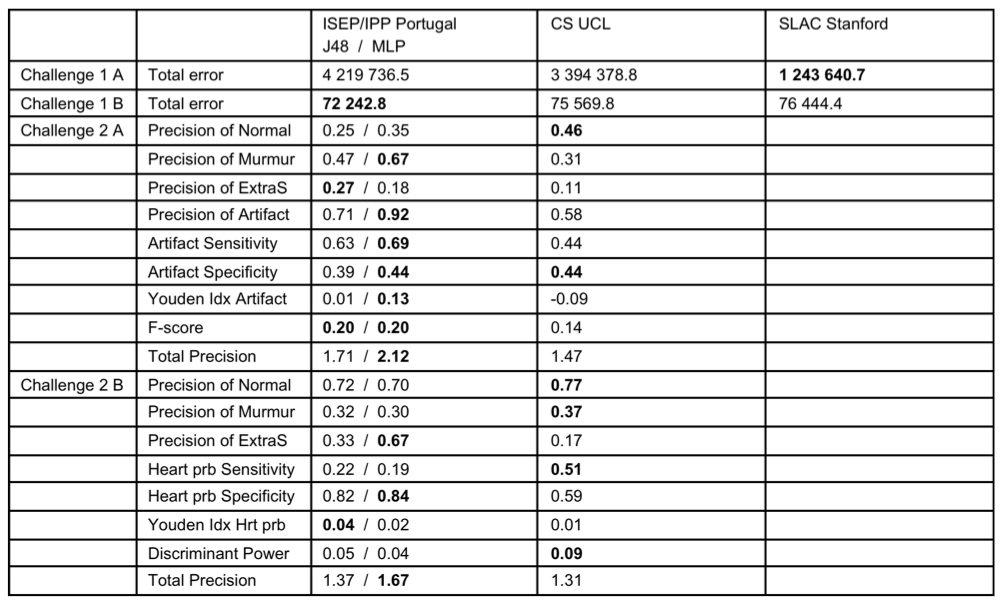
\includegraphics[width=7cm]{challengeresults.png}
\centering
\caption{Results presented in Classifying Heart Sounds Workshop, 2012}
\end{figure}


\end{abstract}

\subsection*{Bibliography}

\begin{verbatim}
http://www.peterjbentley.com/heartchallenge/
\end{verbatim}
\begin{verbatim}
http://cdn.intechopen.com/pdfs/19510/InTech-Computerized_
heart_sounds_analysis.pdf
\end{verbatim}

H. Ryu, J. Park and H. Shin, \textit{\"Classification of heart sound recordings using convolution neural network\"}, 2016 Computing in Cardiology Conference (CinC), Vancouver, BC, 2016, pp. 1153-1156.


\end{document}